%%%%%%%%%%%%%%%%%%%%%%%%%%%%%%%%%%%%%%%%%
% University Assignment Title Page 
% LaTeX Template
% Version 1.0 (27/12/12)
%
% This template has been downloaded from:
% http://www.LaTeXTemplates.com
%
% Original author:
% WikiBooks (http://en.wikibooks.org/wiki/LaTeX/Title Creation)
%
% License:
% CC BY-NC-SA 3.0 (http://creativecommons.org/licenses/by-nc-sa/3.0/)
% 
% Instructions for using this template:
% This title page is capable of being compiled as is. This is not useful for 
% including it in another document. To do this, you have two options: 
%
% 1) Copy/paste everything between \begin{document} and \end{document} 
% starting at \begin{titlepage} and paste this into another LaTeX file where you 
% want your title page.
% OR
% 2) Remove everything outside the \begin{titlepage} and \end{titlepage} and 
% move this file to the same directory as the LaTeX file you wish to add it to. 
% Then add \input{./title page_1.tex} to your LaTeX file where you want your
% title page.
%
%%%%%%%%%%%%%%%%%%%%%%%%%%%%%%%%%%%%%%%%%

%----------------------------------------------------------------------------------------
%	PACKAGES AND OTHER DOCUMENT CONFIGURATIONS
%----------------------------------------------------------------------------------------

\documentclass[12pt]{article}
\usepackage{graphicx}
\usepackage[utf8]{inputenc}  
\usepackage[T1]{fontenc} 
\usepackage[top=1cm,bottom=1cm,left=0.5cm,right=1.5cm,asymmetric]{geometry}
\usepackage{amsfonts}
\usepackage{graphicx}
\usepackage{amsmath}
\usepackage{caption}
\usepackage{subcaption}
\usepackage{float}
\usepackage{subfig}
\usepackage{fancyhdr}
\pagestyle{fancy}
\renewcommand{\footrulewidth}{1pt}
\fancyhead[R]{\textit{Master MVA : Kernel Methods}}
\fancyfoot[L]{\textit{}}
%\usepackage{unicode-math}
%\setmathfont{XITS Math}
%\setmathfont[version=setB,StylisticSet=1]{XITS Math}
\usepackage{array,multirow,makecell}
\setcellgapes{1pt}
\makegapedcells
\newcolumntype{R}[1]{>{\raggedleft\arraybackslash }b{#1}}
\newcolumntype{L}[1]{>{\raggedright\arraybackslash }b{#1}}
\newcolumntype{C}[1]{>{\centering\arraybackslash }b{#1}}

\pagestyle{fancy}
\renewcommand{\footrulewidth}{1pt}
\fancyfoot[L]{\textit{}}
\newcommand{\cond}{(x_i|x_{\pi_i})}

%\usepackage{caption}
%\usepackage{subcaption}


%\usepackage{unicode-math}
%\setmathfont{XITS Math}
%\setmathfont[version=setB,StylisticSet=1]{XITS Math}


%\geometry{hmargin=1.5cm,vmargin=2cm}   

\geometry{hmargin=2.5cm,vmargin=2cm}   
\begin{document}

\section*{Kernel Methods : Homework 2}
\section*{Thibaud Ehret \& Sammy Khalife}
\subsubsection*{01/02/2014}

\section*{1)}
The formula for the projection on the $i^\text{th}$ eigenvector is $ \sum_{j=1}^{n} \alpha^{(i)}_j (\Phi(x_j) - m) $.
\begin{eqnarray*}
	 \sum_{j=1}^{n} \alpha^{(i)}_j (\Phi(x_j) - m) &=&  \sum_{j=1}^{n} \alpha^{(i)}_j \Phi(x_j) -\sum_{j=1}^{n} \alpha^{(i)}_j m\\
	 &=& \sum_{j=1}^{n} \alpha^{(i)}_j \Phi(x_j) - m \left(\sum_{j=1}^{n} \alpha^{(i)}_j\right)\\
	 &=& \sum_{j=1}^{n} \alpha^{(i)}_j \Phi(x_j) - \frac{1}{n} \left( \sum_{u=1}^{n} \Phi(x_u) \right) \left(\sum_{j=1}^{n} \alpha^{(i)}_j\right)\\
	 &=& \sum_{j=1}^{n} \alpha^{(i)}_j \Phi(x_j) -  \left( \sum_{u=1}^{n} \frac{1}{n}\left(\sum_{j=1}^{n} \alpha^{(i)}_j\right)\Phi(x_u) \right)\\ 
	 &=& \sum_{j=1}^{n} \alpha^{(i)}_j \Phi(x_j) -  \left( \sum_{j=1}^{n} \frac{1}{n}\left(\sum_{u=1}^{n} \alpha^{(i)}_u\right)\Phi(x_j) \right)\\ 
	 &=& \sum_{j=1}^{n} \left(\alpha^{(i)}_j - \frac{1}{n}\left(\sum_{u=1}^{n} \alpha^{(i)}_u\right)\right)\Phi(x_j)
\end{eqnarray*}
We note $\beta_j = \alpha^{(i)}_j - \frac{1}{n}\left(\sum_{u=1}^{n} \alpha^{(i)}_u\right)$, so that the vector can be written $ \sum_{j=1}^{n} \beta^{(i)}_j \Phi(x_j)$. 
Therefore after injecting into the expression of $\Psi$,
\begin{eqnarray*}
	\Psi(x) &=& \sum_{i=1}^d \langle \sum_{j=1}^{n} \beta^{(i)}_j \Phi(x_j), \Phi(x) - m\rangle \left(\sum_{j=1}^{n} \beta^{(i)}_j \Phi(x_j) \right)+ m\\
	&=& \sum_{i=1}^d \left(\sum_{j=1}^{n} \beta^{(i)}_j \langle \Phi(x_j), \Phi(x) \rangle\right) \left(\sum_{j=1}^{n}\beta^{(i)}_j \Phi(x_j)\right) - \sum_{i=1}^d \left(\sum_{j=1}^{n} \beta^{(i)}_j \langle \Phi(x_j), m \rangle\right)\left(\sum_{j=1}^{n}\beta^{(i)}_j \Phi(x_j)\right)+ m\\
	&=& \sum_{i=1}^d \left(\sum_{j=1}^{n} \beta^{(i)}_j K(x_j,x)\right) \left(\sum_{j=1}^{n}\beta^{(i)}_j \Phi(x_j)\right) - \sum_{i=1}^d \left(\sum_{j=1}^{n} \beta^{(i)}_j \langle \Phi(x_j), \frac{1}{n}\sum_{u=1}^{n} \Phi(x_u) \rangle\right) \left(\sum_{j=1}^{n}\beta^{(i)}_j \Phi(x_j)\right)\\
	&&+ \frac{1}{n}\sum_{u=1}^{n} \Phi(x_u)\\
	&=& \sum_{i=1}^d \left(\sum_{j=1}^{n} \beta^{(i)}_j K(x_j,x)\right) \left(\sum_{j=1}^{n}\beta^{(i)}_j \Phi(x_j)\right) - \sum_{i=1}^d \left(\sum_{j=1}^{n} \beta^{(i)}_j \frac{1}{n}\sum_{u=1}^{n} K(x_j,x_u)\right) \left(\sum_{j=1}^{n}\beta^{(i)}_j \Phi(x_j)\right)\\
	&&+ \frac{1}{n}\sum_{u=1}^{n} \Phi(x_u)\\
	&=& \sum_{i=1}^d \left(\sum_{j=1}^{n} \beta^{(i)}_j K(x_j,x)\right) \left(\sum_{j=1}^{n}\beta^{(i)}_j \Phi(x_j)\right) - \sum_{i=1}^d \left(\sum_{j=1}^{n} \beta^{(i)}_j \frac{1}{n}\sum_{u=1}^{n} K(x_j,x_u)\right) \left(\sum_{j=1}^{n}\beta^{(i)}_j \Phi(x_j)\right)\\
	&&+ \frac{1}{n}\sum_{u=1}^{n} \Phi(x_u)\\
	&=& \sum_{j=1}^n \left( \sum_{u=1}^{n} \left(\sum_{i=1}^{d}\beta^{(i)}_u \beta^{(i)}_j\right) K(x_u,x) - \sum_{u=1}^{n} \left(\sum_{i=1}^{d}\beta^{(i)}_u \beta^{(i)}_j\right) \left(\frac{1}{n} \sum_{v=1}^n K(x_u,x_v)\right) + \frac{1}{n} \right) \Phi(x_j)
\end{eqnarray*}

Therefore 
\[\gamma_j = \sum_{u=1}^{n} \left(\sum_{i=1}^{d}\beta^{(i)}_u \beta^{(i)}_j\right) \left(K(x_u,x) - \left(\frac{1}{n} \sum_{v=1}^n K(x_u,x_v)\right)\right) + \frac{1}{n} \]


\section*{2)}

\begin{eqnarray*}
	f(y) &=& \|\Phi(y) - \Psi(x) \|^2\\
	&=& \langle \Phi(y) - \Psi(x), \Phi(y) - \Psi(x) \rangle \\
	&=& \langle \Phi(y), \Phi(y) \rangle -  2 \langle \Phi(y), \Psi(x) \rangle + \langle \Psi(x), \Psi(x) \rangle\\
	&=& K(y,y) -  2 \langle \Phi(y), \Psi(x) \rangle + \langle \Psi(x), \Psi(x) \rangle
\end{eqnarray*}

Using the the fact that $\Psi(x) = \sum_{i=1}^n \gamma_i \Phi(x_i)$,
\begin{eqnarray*}
	f(y) &=& K(y,y) - 2\langle \Phi(y), \sum_{i=1}^n \gamma_i \Phi(x_i \rangle + \langle \sum_{i=1}^n \gamma_i \Phi(x_i), \sum_{i=1}^n \gamma_i \Phi(x_i) \rangle \\
	&=& K(y,y) - 2\sum_{i=1}^n \gamma_i \langle \Phi(y), \Phi(x_i) \rangle + \sum_{i=1}^n \sum_{j=1}^n \gamma_i\gamma_j\langle  \Phi(x_i),  \Phi(x_j) \rangle \\
	&=& K(y,y) - 2\sum_{i=1}^n \gamma_i K(y,x_i) + \sum_{i=1}^n \sum_{j=1}^n \gamma_i\gamma_j K(x_i,x_j)
\end{eqnarray*}

The idea behind $\Psi(x)$ is to denoise $x$ in the feature space, by keeping only the participation over the $d$ first principal components we can hope to have consider the signal without its noise. Therefore ooptimizing $f(y)$ corresponds to finding the best $y$ in the original space such that it is as close as possible to the ``denoised`` version in the feature space, therefore the $y$ that optimizes $f$ for a given $x$ correspond to the best denoised version in the original space.

\section*{3)}
In the case of $K(x,x')=exp(-\frac{||x-x'||^{2}}{2\sigma^{2}})$,
$$f(y)=\sum_{i=1}^{n}\sum_{j=1}^{n}\gamma_{i}\gamma_{j}exp(-\frac{||x_{i}-x'_{j}||^{2}}{2\sigma^{2}})-2\sum_{i=1}^{n}\gamma_{i}exp(-\frac{||y-x_{i}||^{2}}{2\sigma^{2}})$$
$$\nabla f(y)=\frac{2}{\sigma^{2}}\sum_{i=1}^{n}(y-x_{i})\gamma_{i}exp(-\frac{||y-x_{i}||^{2}}{2\sigma^{2}})$$
We can here use a gradient descent method to find local minimum of f. We see that a stationary point satisfies : 
$$y=\frac{\sum_{i=1}^{n}x_{i}\gamma_{i}exp(-\frac{||y-x_{i}||^{2})}{2\sigma^{2}})}{\sum_{i=1}^{n}\gamma_{i}exp(\frac{-||y-x_{i}||^{2})}{2\sigma^{2}})}$$
We can apply a fixed point method :

$$y_{k+1}=\frac{\sum_{i=1}^{n}x_{i}\gamma_{i}exp(-\frac{||y_{k}-x_{i}||^{2})}{2\sigma^{2}})}{\sum_{i=1}^{n}\gamma_{i}exp(\frac{-||y_{k}-x_{i}||^{2})}{2\sigma^{2}})}$$
With initialization at different points.~\\
~\\
Or we can use the Newton step with the Hessian :
$$H_{f}(y)=\frac{2}{\sigma^{2}} \sum_{i=1}^{n}\gamma_{i}exp(-\frac{||y-x_{i}||^{2}}{2\sigma^{2}})[\frac{Id}{n}-(y-x_{i})(y-x_{i})^{t} ]$$

$$y_{k+1}=y_{k}-H_{f}^{-1}(y_{k})\nabla y_{k}$$

~\\
~\\
\section*{4)} Data used : (http://statweb.stanford.edu/~tibs/ElemStatLearn/datasets/zip.info.txt)
~\\
~\\
This dataset is composed of normalized handwritten digits, automatically scanned from envelopes by the U.S. Postal Service. The original
scanned digits are binary and of different sizes and orientations; the
images  here have been deslanted and size normalized, resulting
in 16 x 16 grayscale images.

We represent in figures \ref{fig:linker}, \ref{fig:polker},\ref{fig:gaussker} and \ref{fig:gaussker2} the projection on the first 2 dimensions for the linear kernel, the polynomial kernel (with $p=2$) and the gaussian kernel with parameter $\sigma = 0.5$ and $\sigma = 1$ respectively.
\begin{figure}[H]
	\minipage{0.4\textwidth}
	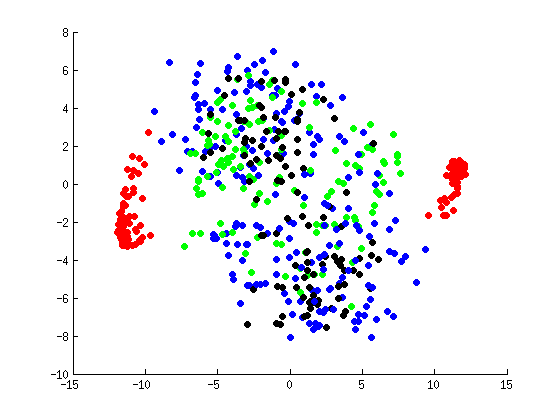
\includegraphics[width=9cm]{linKernel.png}
	\subcaption{Linear kernel}\label{fig:linker}
	\endminipage\hfill
	\minipage{0.4\textwidth}
	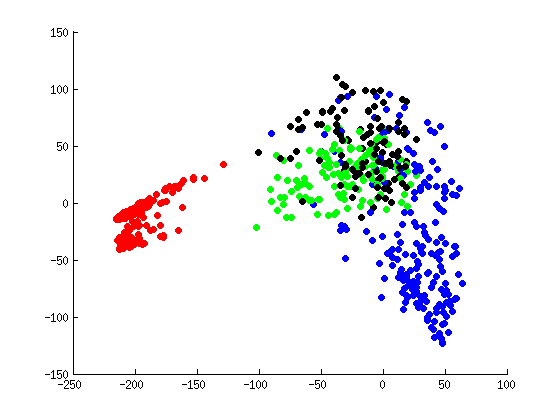
\includegraphics[width=9cm]{polyKernel.png}
	\subcaption{Polynomial kernel}\label{fig:polker}
	\endminipage \\
	\minipage{0.4\textwidth}
	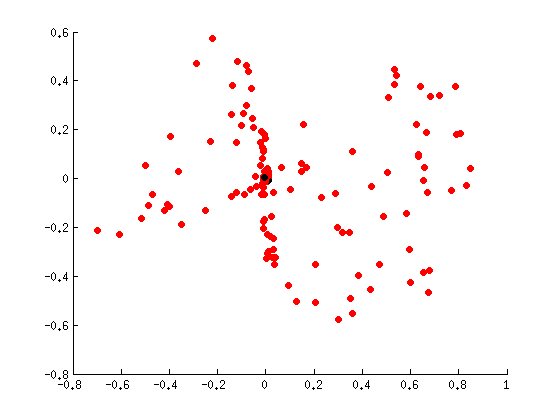
\includegraphics[width=9cm]{gaussianKernel.png}
	\subcaption{Gaussian kernel with $\sigma = 0.5$}\label{fig:gaussker}
	\endminipage \hfill
	\minipage{0.4\textwidth}
	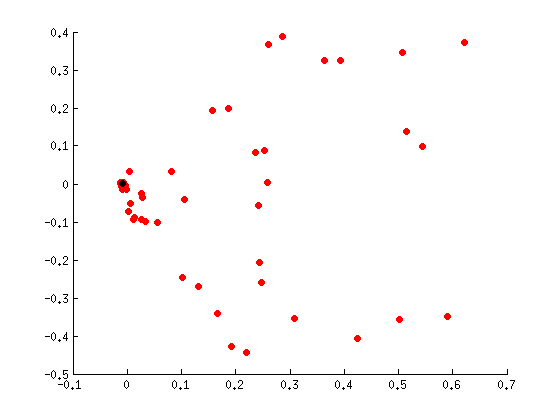
\includegraphics[width=9cm]{gaussianKernel2.png}
	\subcaption{Gaussian kernel with $\sigma = 1$}\label{fig:gaussker2}
	\endminipage \hfill
	\caption{Visualization for different kernels, the class of $0$ is in blue, the class of $1$ is in red, the class of $2$ is in green and the class of $3$ is in black}
\end{figure} 
%\linewidth
\begin{figure}[H]
	\minipage{0.4\textwidth}
	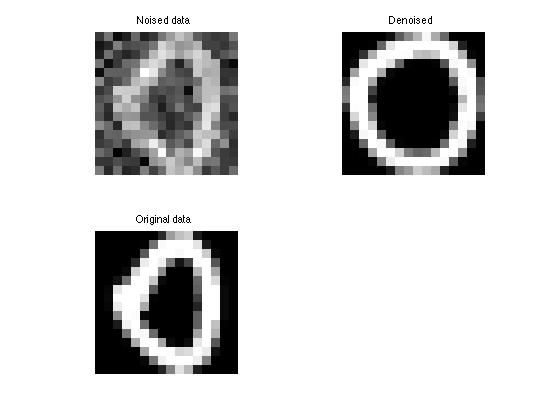
\includegraphics[width=9cm]{result0.jpg}
	\subcaption{}\label{fig:awesome_image1}
	\endminipage\hfill
	\minipage{0.4\textwidth}
	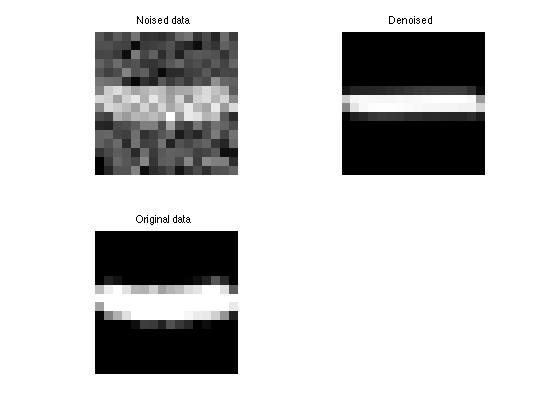
\includegraphics[width=9cm]{result1.jpg}
	\subcaption{}\label{fig:awesome_image2}
	\endminipage \\
	\minipage{0.4\textwidth}
	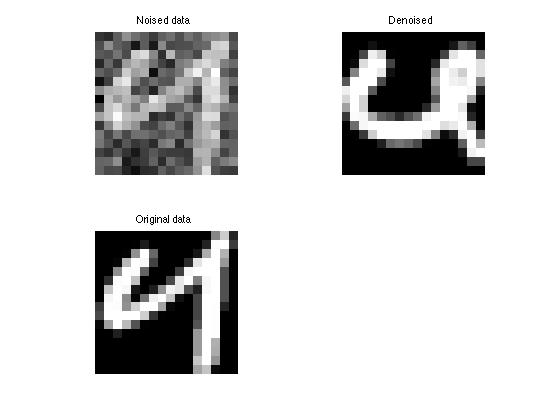
\includegraphics[width=9cm]{result2.jpg}
	\subcaption{}\label{fig:awesome_image3}
	\endminipage \hfill
	\minipage{0.4\textwidth}
	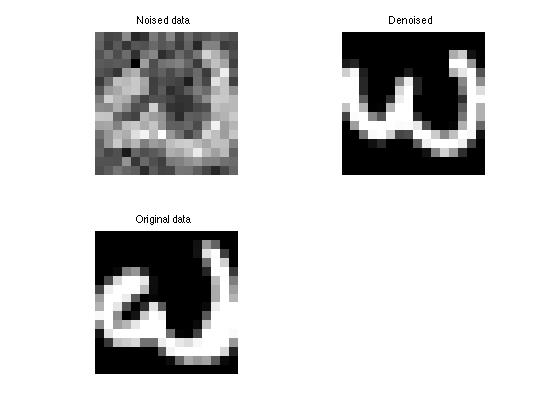
\includegraphics[width=9cm]{result3.jpg}
	\subcaption{}\label{fig:awesome_image4}
	\endminipage
	\caption{Results on different digits}
\end{figure} 
These results have been obtained with \textbf{100 training samples}, and with \textbf{d=50}. We see that the minimization process that projects the noised data over the vector spanned by the eigenvectors simplify the geometry. Increasing d does not help to achieve better denoising, since we  are closer and closer to the noised data x :

\begin{figure}[H]
	\minipage{0.4\textwidth}
	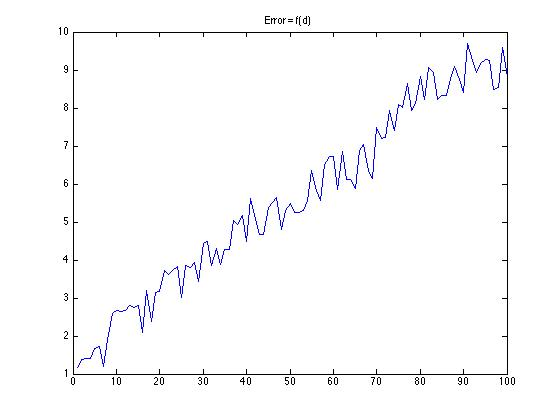
\includegraphics[width=7cm]{plotError.jpg}
	\subcaption{Error plot as a function of d}\label{fig:awesome_image5}
	\endminipage\hfill
\end{figure}

\end{document}
